\documentclass[journal,10pt,twocolumn]{article}
\usepackage[margin=0.5in]{geometry}
\usepackage[cmex10]{amsmath}
\usepackage{amsmath}
\usepackage{array}
\usepackage{booktabs}
% The preceding line is only needed to identify funding in the first footnote. If that is unneeded, please comment it out.
\usepackage{cite}
\usepackage{amsmath,amssymb,amsfonts}
\usepackage{graphicx}
\usepackage{textcomp}
\usepackage{xcolor}
\graphicspath{{./figs/}}{}
\usepackage{amsmath,amssymb,amsfonts,amsthm}
\usepackage{gensymb}
\newcommand{\myvec}[1]{\ensuremath{\begin{pmatrix}#1\end{pmatrix}}}
\let\vec\mathbf
\title{
Conic Assignment
}
\author{GINNA SHREYANI}
\providecommand{\norm}[1]{\left\lVert#1\right\rVert}
\providecommand{\abs}[1]{\left\vert#1\right\vert}
\let\vec\mathbf
%\newcommand{\myvec}[1]{\ensuremath{\begin{pmatrix}#1\end{pmatrix}}}
\newcommand{\mydet}[1]{\ensuremath{\begin{vmatrix}#1\end{vmatrix}}}
\providecommand{\brak}[1]{\ensuremath{\left(#1\right)}}
\providecommand{\brak}[1]{\ensuremath{\left(#1\right)}}
\providecommand{\lbrak}[1]{\ensuremath{\left(#1\right.}}
\providecommand{\rbrak}[1]{\ensuremath{\left.#1\right)}}
\providecommand{\sbrak}[1]{\ensuremath{{}\left[#1\right]}}

\begin{document}
\maketitle
\tableofcontents
\bigskip
\section{Problem Statement}
Show that the locus of a point that divides a chord joining the points P and Q(0,0) of the parabola $y^2 = 4x$ internally in the ratio 1:3 is a parabola.Find the vertex of a parabola.\\
\section{Solution}
Let $\vec{X}$ be Locus point that divides the chord joining  $\vec{P}$ and $\vec{Q}$ internally in the ratio 1:3.  \\


The given equation of parabola $y^2 = 4x$ can be written in the general quadratic form as
\begin{align}
    \vec{x}^{\top}\vec{V}\vec{x}+2\vec{u}^{\top}\vec{x}+f=0
    \label{eq-1}
\end{align}
where
\begin{align}
	\label{eq:V_matrix}
	\vec{V} &= \myvec{0 & 0\\0 & 1},\\
	\label{eq:u_vector}
	\vec{u} &= \myvec{-2\\0},\\
	\label{eq:f_value}
	f &= 0
\end{align}

By section formula the point that divides the  line joining $\vec{P}$ and $\vec{Q}$ as $\vec{X}$ is:
 
\begin{equation}
	\vec{X}=\frac{\vec{Q}+3\vec{P}}{4}
	 \label{eq-4}
\end{equation}
\\
 \begin{equation}
	\vec{P}=\frac{4\vec{X}-\vec{Q}}{3}
	 \label{eq-5}
\end{equation}
Substituting P in ($\ref{eq-1}$), we get
\begin{align}
&\vec{P^T}\vec{V}\vec{P}+2\vec{u^T}\vec{P}+f = 0
\label{eq-6}
\end{align}

Substituting ($\ref{eq-5}$) in ($\ref{eq-6}$), We get 

\begin{multline}
    (\frac{4\vec{X}-\vec{Q}}{3})^{\top}\vec{V}(\frac{4\vec{X}-\vec{Q}}{3})+2\vec{u}^{\top}(\frac{4\vec{X}-\vec{Q}}{3})=0
     \label{eq-8}
    \end{multline}

\begin{multline}
    \label{eq:conic_quad_form}
    \frac{1}{9}(4\vec{X}^{\top}\vec{V}4\vec{X}-4\vec{X}^{\top}\vec{V}\vec{Q}-\vec{Q}^{\top}\vec{V}4\vec{X}+\vec{Q}^{\top}\vec{V}\vec{Q}) + \frac{2}{3}\vec{u}^{\top}4\vec{X}-\frac{2}{3}\vec{u}^{\top}\vec{Q}
    \end{multline}

\begin{multline}
    \label{eq:conic_quad_form}
	\frac{16}{9}\vec{X}^{\top}\vec{V}\vec{X}-\frac{4}{9}\vec{X}^{\top}\vec{V}\vec{Q}-\frac{4}{9}\vec{Q}^{\top}\vec{V}\vec{X}+\frac{1}{9}\vec{Q}^{\top}\vec{V}\vec{Q}+\frac{8}{3}\vec{u}^{\top}\vec{X}-\frac{2}{3}\vec{u}^{\top}\vec{Q}=0
    \end{multline}
 
\begin{align*}
    \label{eq:conic_quad_form}
	&\frac{16}{9}\vec{X}^{\top}\vec{V}\vec{X}+\frac{8}{3}\vec{u}^{\top}\vec{X}=0
    \end{align*}
        
\begin{equation}
    \label{eq:conic_quad_form}
	\vec{X}^{\top}\vec{V}\vec{X}+2\vec{u'}^{\top}\vec{X}=0
\end{equation}
where
\begin{align}
	\vec{V} &= \myvec{0 & 0\\0 & 1}\\
	\vec{u'} &=\myvec{-3/2\\0}\\
\end{align}
{\begin{table}[h]
    \centering
    \begin{tabular}{|c|c|c|}
       \hline
       \textbf{Symbol}&\textbf{Value}&\textbf{Description}  \\
       \hline
	    $\vec{Q}$ & $\myvec{
		    0\\
		    0}$
	    & given point\\
        \hline
	    $\vec{P}$ & $\myvec{x\\y}$
 &  point on given locus \\
        \hline
	    $\vec{X}$ & $\myvec{x\\y}$
 & divides in the ratio 1:3 $\vec{PQ}$  \\
       \hline
    \end{tabular}
    \caption{Parameters}
    \label{tab:my_label}
\end{table}

\begin{figure}[h]
    \centering
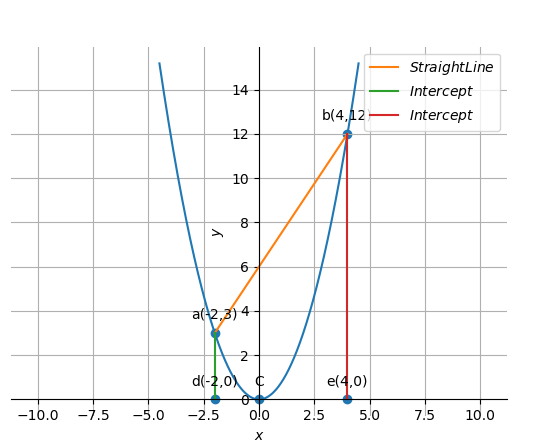
\includegraphics[width=\columnwidth]{fig/conic.png}
    \caption{Found the locus equation }
    \label{fig:my_label}
\end{figure}

}
\end{document}

